\documentclass[11pt]{scrartcl}
\usepackage[utf8]{inputenc}
\usepackage[sexy]{evanchen} 
\usepackage{graphicx}
\graphicspath{{8 Outsource K Math/Gambar/}}

\title{Kekongruenan dan Kesebangunan}
\author{Azzam and Akeyla}
\date{Maret 2023}

\begin{document}

\maketitle

\renewcommand*\contentsname{Daftar Isi}
\tableofcontents

\newpage

\section{Kekongruenan}
\begin{figure}[!h]
    \centering
    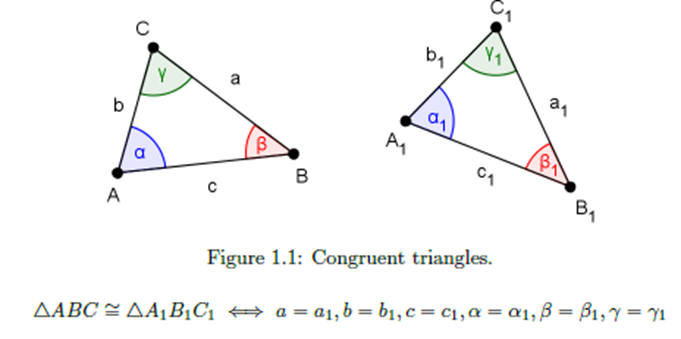
\includegraphics{Kongruen.png}
    \caption{Dua segitiga yang kongruen}
    \label{fig:my_label}
\end{figure}
Dua buah segitiga dikatakan kongruen ketika besar sudut dan panjang sisi mereka yang saling berkoresponden sama. \\
Dalam soal, biasanya hanya sebagian kuantitas saja yang diketahui. Untuk membuktikan kekongruenan, bisa digunakan salah satu dari tiga kriteria berikut:
\begin{enumerate}
    \item Kriteria SSS (side-side-side) \\
    Jika ketiga pasang sisi yang saling berkorespondensi memiliki panjang yang sama, maka kedua segitiga kongruen.
    \item Kriteria SAS (side-angle-side) \\
    Jika dua pasang sisi yang saling berkorespondensi memiliki panjang yang sama dan besar sepasang sudut yang diapit kedua sisi tersebut juga sama, maka kedua segitiga tersebut kongruen.
    \item Kriteria ASA (angle-side-angle) \\
    Jika dua pasang sudut yang saling berkorespondensi memiliki besar yang sama dan panjang sepasang sisi yang menghubungkan kedua sudut tersebut juga sama, maka kedua segitiga tersebut kongruen.  
\end{enumerate}

\section{Kesebangunan}
\begin{figure}[!h]
    \centering
    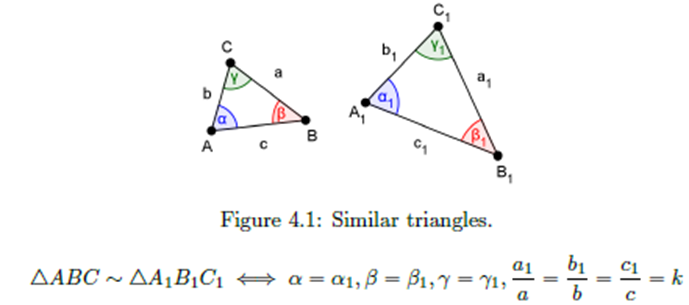
\includegraphics{Sebangun.png}
    \caption{Dua segitiga yang sebangun}
    \label{fig:my_label}
\end{figure}
Dua segitiga dikatakan sebangun jika besar sudut yang saling berkorespondensi sama dan panjang sisi yang saling berkorespondensi proporsional.\\
Dalam soal, biasanya hanya sebagian kuantitas saja yang diketahui. Untuk membuktikan kesebangunan, bisa digunakan salah satu dari tiga kriteria berikut:
\begin{enumerate}
    \item Kriteria AA (angle-angle)\\
    Jika dua pasang sudut yang saling berkorespondensi memiliki besar yang sama, maka kedua segitiga sebangun.
    \item Kriteria SSS (side-side-side) \\
    Jika tiga pasang sisi yang saling berkorespondensi proporsional, maka kedua segitiga sebangun.    
    \item Kriteria SAS (side-angle-side) \\
    Jika dua pasang sisi yang saling berkorespondensi proporisonal dan sepasang sudut yang diapit kedua pasang sisi tersbeut besarnya sama, maka kedua segitiga sebangun.
\end{enumerate}
Patut diingat bahwa rasio $k$ juga menunjukkan perbandingan panjang segmen-segmen garis lain antara kedua segitiga, seperti garis tinggi, garis median, garis bagi, dan seterusnya. Adapun, perbandingan luas kedua segitiga tersebut adalah $k^2$.


\section{Latihan}
\begin{problem}
    (OSK 2022 Kemampuan Dasar) Diberikan segitiga $ABC$ siku-siku di $B$. Titik $D$ berada pada sisi $AB$ dan titik $E$ berada pada sisi $AC$. Diketahui $DE$ sejajar $BC$. Jika $AD = 21, DB = 3,$ dan $BC = 32$, maka panjang $AE$ adalah ...
\end{problem}

\begin{problem}
    (OSK 2022 Kemampuan Dasar) Diberikan sebuah segitiga $ABC$ yang siku-siku di $B$. Diketahui bahwa $AB = 2BC$ dan $BD = CD$. Jika luas segitiga $DEC$ adalah $10$, luas dari segitiga $AFE$ adalah ...
\end{problem}

\begin{problem}
    (OSK 2021 Kemampuan Dasar) Pada gambar ini sebuah persegi panjang dibagi menjadi dua buah persegi yang panjang sisinya $6$. Luas total daerah yang diarsir adalah ...
    \begin{figure}[h]
        \centering
        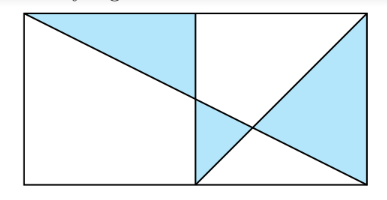
\includegraphics{OSK20216KD.png}
        \label{fig:my_label}
    \end{figure}
\end{problem}


\begin{problem}
%https://artofproblemsolving.com/community/c5h1588241p9833164
%24
(AMC 10 2018) Pada gambar di bawah, seluruh segitiga yang ada akan sebangun dengan segitiga sama kaki $ABC$ dengan $AB = AC$. Diketahui bahwa luas masing-masing segitiga terkecil sama dengan $1$ dan luas segitiga $ABC$ adalah $40$. Luas trapesium $DBCE$ adalah ...
\begin{figure}[h]
    \centering
    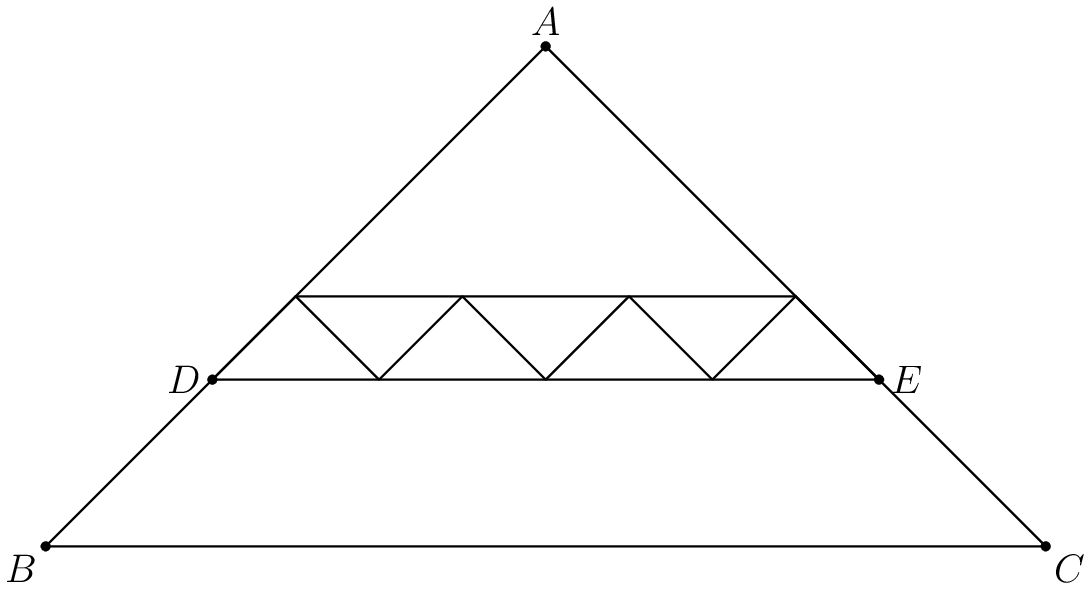
\includegraphics[width=0.5\linewidth]{AMC201810A9.png}
\end{figure}
\end{problem}

\begin{problem}
    (Denmark MO 2022) Persegi $ABCD$ memiliki panjang sisi $1$, Titik $E$ terletak di segmen garis $CD$. Sinar $AE$ memotong $BC$ di titik $F$. Tentukan nilai dari $\dfrac{1}{AE^2} + \dfrac{1}{AF^2}$
\end{problem}

\end{document}